% Provenance (never printed): see sources/outline_sources.md (Year 2: climate archives and proxies;
% foraminiferal and ice isotopes; Mg/Ca; pollen; speleothems; tree rings; dating the archives).
% Calibrations after Miller et al. (2020), Groeneveld et al. (2019) and Morley et al. (2024); ice
% cores after White (Geochemistry, ch. 9), Werner et al. (2018) and the EPICA Dome C file of Jouzel
% et al. (2007); age model after Svensson et al. (2008); deep-water context after Wharton et al.
% (2026); figures from figdata/bachelor-2/proxies.py (data/derived lr04, edc-temperature,
% co2-icecore); values of the exercises and problem computed in the Book 4 scratch calculator
% calc/ch24.py.
\chapter{Archives climatiques et indicateurs}\label{ch:b2:climate-proxies}

En 1955, un jeune géochimiste publie les rapports isotopiques de l'oxygène des minuscules coquilles de
foraminifères prélevées dans des carottes du fond océanique, et il y trouve quinze cycles glaciaire--interglaciaire
sur les \num{600000} dernières années. Il les lit surtout comme des températures : il n'attribue qu'environ un
cinquième des variations à la glace stockée sur les continents. Dix-huit ans plus tard, Shackleton et Opdyke
concluent le contraire : l'effet principal est le stockage d'eau isotopiquement légère dans les inlandsis. Les mêmes
coquilles, les mêmes nombres, deux lectures. Une coquille de calcite enregistre la température de l'eau dans
laquelle elle s'est formée et la composition de cette eau, et la composition de l'eau de mer dépend de la quantité
de glace présente sur les continents. Ce chapitre porte sur de tels enregistrements, sur les archives qui les conservent,
sur les indicateurs lus dans ces archives, sur la manière dont ils sont calibrés face aux thermomètres et dont ils sont
datés, et sur l'art de distinguer deux signaux portés par une même coquille.
% ledger: white13c9:paleo-history

\begin{recall}
\textbf{Des volumes scolaires}~: \omterm{def:b2:climate-proxies:proxy}{archive climatique} et indicateur, carotte de glace, période glaciaire et
interglaciaire, dernier maximum glaciaire (il y a environ \num{23000} à \num{19000} ans), analyse
pollinique. \textbf{Du volume de première année}~: datation radiométrique, âge radiocarbone et sa
courbe de calibration~; boue calcaire, faite de coccolithes et de coquilles de foraminifères.
\textbf{Du \cref{ch:b2:isotope-geochemistry}}~: les \omterm{def:b2:isotope-geochemistry:standards}{étalons isotopiques de référence} \omterm{def:b2:isotope-geochemistry:standards}{VSMOW} et \omterm{def:b2:isotope-geochemistry:standards}{VPDB}
(\cref{def:b2:isotope-geochemistry:standards}) et la \omterm{prop:b2:isotope-geochemistry:mwl}{droite des eaux météoriques}, $\delta\mathrm{D}
\approx 8\,\delta^{18}\mathrm{O} + 10$ (\cref{prop:b2:isotope-geochemistry:mwl}). \textbf{Des volumes de
chimie}~: la valeur $\delta$ et le facteur de fractionnement. \textbf{Des volumes de mathématiques}~:
la droite des moindres carrés.
\end{recall}
% ledger: ipcc:lgm-cooling, kc98:mwl, kc98:standards

\section{Archives et indicateurs}\label{sec:b2:climate-proxies:archives}

Les instruments n'ont mesuré le climat que récemment. Tout ce qui est antérieur se lit dans des matériaux
qui se sont formés ou déposés couche après couche pendant que le climat agissait sur eux : neige devenue glace sur
les inlandsis polaires, coquilles tombant sur le fond des océans, cernes des arbres, coraux, dépôts des
grottes, boue des lacs. Les volumes scolaires appelaient ces matériaux des archives, et les grandeurs
mesurées dans eux des indicateurs ; il nous faut des mots plus précis.

\begin{definition}[Archive climatique~; indicateur climatique]\label{def:b2:climate-proxies:proxy}
Une \emph{archive climatique}\index{archive climatique} est un matériau naturel qui s'accumule
progressivement, couche sur couche ou anneau sur anneau, et conserve des caractères physiques, chimiques ou biologiques
du milieu dans lequel chaque partie s'est formée. Un \emph{indicateur
climatique}\index{indicateur climatique} est une grandeur mesurée dans une archive qui dépend d'une variable
climatique, comme une température, une quantité de pluie ou un volume de glace, par une relation qui peut être
calibrée, et qui tient ainsi lieu d'une mesure de cette variable, qui n'a jamais été faite.
\end{definition}
% ledger: ncei:proxy, ncei:paleocean

Trois propriétés décident de ce qu'une archive peut dire : sa résolution (la durée couverte par un échantillon),
sa portée (jusqu'où elle remonte) et la manière dont elle est datée. Une archive à couches annuelles peut être lue
année après année et datée par comptage ; les autres demandent des âges radiométriques ou une comparaison avec un
enregistrement daté. Le tableau ci-dessous compare les archives de ce chapitre.

\begin{center}
\small
\begin{tabular}{>{\raggedright\arraybackslash}p{0.17\linewidth}>{\raggedright\arraybackslash}p{0.27\linewidth}>{\raggedright\arraybackslash}p{0.21\linewidth}>{\raggedright\arraybackslash}p{0.24\linewidth}}
\hline
archive & indicateurs de ce chapitre & couches annuelles & datation \\
\hline
sédiment océanique profond & $\delta^{18}$O et Mg/Ca des foraminifères & non & radiocarbone, comparaison avec des
enregistrements datés \\
glace polaire & $\delta$D et $\delta^{18}$O de la glace, air emprisonné dans les bulles & dans la partie haute des
carottes épaisses & comptage des couches, couches volcaniques datées \\
cernes d'arbres & largeur des cernes, densité du bois, isotopes & oui & comptage et \omterm{def:b2:climate-proxies:dendro}{interdatation} des cernes \\
\omterm{def:b2:climate-proxies:archives}{spéléothèmes} & $\delta^{18}$O & dans certains cas & datation radiométrique \\
sédiments lacustres & \omterm{def:b2:climate-proxies:archives}{varves}, pollen & là où il y a des \omterm{def:b2:climate-proxies:archives}{varves} & comptage des \omterm{def:b2:climate-proxies:archives}{varves} \\
\hline
\end{tabular}
\end{center}
% ledger: ncei:proxy, ncei:paleocean, ncei:tree-ring, ncei:speleothem, mccarthy23:varves, svensson08:gicc05, noaa:gisp2-layers, bebchuk26:crossdating

Un indicateur n'est jamais la mesure pure d'une seule variable. La largeur d'un cerne d'arbre dépend de la chaleur
de l'été et de la pluie ; le $\delta^{18}$O d'une coquille, de la température de l'eau et de sa
composition isotopique. Le travail du paléoclimatologue consiste à trouver un indicateur dont la dépendance
à la variable recherchée est forte et connue, à mesurer indépendamment les autres influences, et à
dater l'échantillon.

\section{Isotopes de l'oxygène dans les coquilles carbonatées}\label{sec:b2:climate-proxies:oxygen}

Les foraminifères sont des protistes unicellulaires, dont beaucoup bâtissent une coquille de calcite ; les espèces
planctoniques flottent dans les eaux de surface, les espèces benthiques vivent sur le fond ou dans le sédiment marin.
Leurs coquilles s'accumulent dans les boues calcaires du volume de première année, et le $\delta^{18}$O de la
calcite se mesure sur quelques coquilles prélevées dans chaque centimètre d'une
carotte.
% ledger: ucmp:forams, ncei:paleocean

\begin{history}[Deux lectures d'un même enregistrement]
Urey calcule en 1947 comment le fractionnement de l'oxygène entre calcite et eau dépend de la température,
et propose que les carbonates enregistrent la température à laquelle ils se forment. Cesare Emiliani, alors son
étudiant, mesure le $\delta^{18}$O de foraminifères prélevés dans des carottes à pistons des océans du monde et publie
en 1955 un enregistrement de 15 cycles glaciaire--interglaciaire sur \num{600000} ans, et attribue pour environ
\qty{20}{\percent} la variation au volume de la glace. En 1973, Shackleton et Opdyke concluent que le stockage
d'eau isotopiquement légère dans les inlandsis est l'effet principal. Les effets vitaux, c'est-à-dire les écarts
d'une espèce à l'équilibre, et l'échange d'oxygène avec l'eau interstitielle après l'enfouissement ne sont en
général pas très importants pour les coquilles des derniers millions d'années ; c'est la composition isotopique
de l'eau qui compte.
\end{history}
% ledger: white13c9:paleo-history

\subsection*{Température}

La calcite qui croît en équilibre avec l'eau est plus riche en \textsuperscript{18}O que l'eau,
et plus l'eau est froide, plus cet enrichissement est grand, comme le montre le calcul d'Urey. Plusieurs
calibrations empiriques relient
la température à la différence entre le $\delta^{18}$O de la calcite, sur l'échelle \omterm{def:b2:isotope-geochemistry:standards}{VPDB}, et
celui de l'eau, sur l'échelle \omterm{def:b2:isotope-geochemistry:standards}{VSMOW}. Pour la mer profonde, on utilise une forme simplifiée pour les coquilles
benthiques.

\begin{proposition}[Une calibration benthique]\label{prop:b2:climate-proxies:benthic}
Pour les foraminifères benthiques aux températures profondes (inférieures à environ \qty{13}{\celsius}),
\[
  T = 16.1 - 4.76\,\bigl[\delta^{18}\mathrm{O}_{\mathrm{b}} - (\delta^{18}\mathrm{O}_{\mathrm{sw}} -
  0.27)\bigr],
\]
avec $T$ en \unit{\celsius}, $\delta^{18}\mathrm{O}_{\mathrm{b}}$ la valeur de la coquille (pour mille,
\omterm{def:b2:isotope-geochemistry:standards}{VPDB}) et $\delta^{18}\mathrm{O}_{\mathrm{sw}}$ celle de l'eau de mer (pour mille, \omterm{def:b2:isotope-geochemistry:standards}{VSMOW}) ; le terme
0.27 convertit l'eau à l'échelle de la calcite. Un refroidissement de \qty{1}{\celsius} à composition d'eau constante élève
$\delta^{18}\mathrm{O}_{\mathrm{b}}$ de $1/4.76 = 0.21$ pour mille.
\end{proposition}
\admitted
% ledger: miller20:paleotemp, groeneveld19:anand

L'équation plus complète dont celle-ci est une simplification comporte un petit terme quadratique,
$T = 16.1 - 4.64x + 0.09x^2$ avec $x$ la différence des deux valeurs $\delta$ ; les coquilles planctoniques
ont leurs propres calibrations, de même forme, par exemple $T = 14.9 - 4.8\,[\delta^{18}\mathrm{O} -
(\delta^{18}\mathrm{O}_{\mathrm{sw}} - 0.27)]$. Toutes partagent une même difficulté : la coquille donne un seul
nombre, $\delta^{18}\mathrm{O}_{\mathrm{b}}$, et l'équation a deux inconnues, $T$ et
$\delta^{18}\mathrm{O}_{\mathrm{sw}}$. Un second indicateur, indépendant, est nécessaire pour les séparer.
% ledger: miller20:paleotemp, groeneveld19:anand

\subsection*{L'effet de volume des glaces}

L'eau qui s'évapore de la mer emporte moins de \textsuperscript{18}O que la mer ; la vapeur, en se déplaçant vers
les pôles et en pleuvant ou en neigeant, s'appauvrit encore, et la neige qui bâtit les inlandsis compte parmi
les eaux les plus légères de la planète : la glace du Groenland a un $\delta^{18}$O de $-30$ à $-35$
pour mille, celle de l'Antarctique descend jusqu'à $-50$. Lorsque les inlandsis croissent, l'isotope léger est
retenu sur les continents, et l'océan qui reste s'alourdit.
% ledger: nasaeo:o18, white:d18o

\begin{definition}[Effet de volume des glaces]\label{def:b2:climate-proxies:ice-volume}
L'\emph{effet de volume des glaces}\index{effet de volume des glaces} est la variation de la composition isotopique en oxygène
de l'océan entier, causée par la croissance ou la fonte des inlandsis continentaux, qui stockent une eau appauvrie
en \textsuperscript{18}O ; il déplace le $\delta^{18}$O de chaque carbonate formé dans la mer de la même quantité,
quelle que soit la température.
\end{definition}
% ledger: nasaeo:o18, white13c9:ice-volume, miller20:paleotemp

\begin{omfigure}
\centering
\begin{tikzpicture}[font=\scriptsize, >=Stealth]
  \foreach \col/\title in {0/{a\enspace aujourd'hui}, 7.0/{b\enspace maximum glaciaire}} {
  \begin{scope}[shift={(\col,0)}]
  \node[anchor=south west] at (0,3.3) {\textbf{\title}};
  \fill[brown!30] (3.6,0) -- (6.4,0) -- (6.4,1.6) -- (3.6,1.2) -- cycle;
  \end{scope}
}
% today: full ocean, small ice sheet
\fill[ocBlue!25] (0,0) rectangle (3.6,1.2);
\node[align=center] at (1.75,0.55) {océan\\$\delta^{18}\mathrm{O} = 0$};
\fill[white, draw=black!50] (5.2,1.43) .. controls (5.6,1.95) and (6.2,1.95) .. (6.4,1.6) -- cycle;
\node at (5.0,0.65) {glace, $-40$};
\draw[black!50] (5.0,0.85) -- (5.7,1.55);
\draw[->, thick, ocBlue] (1.6,1.35) .. controls (2.4,2.9) and (4.6,2.9) .. (5.6,2.05);
\node at (3.4,3.0) {vapeur, légère};
% glacial: lower sea, big ice sheet
\begin{scope}[shift={(7.0,0)}]
\fill[ocBlue!35] (0,0) rectangle (3.6,0.85);
\draw[densely dashed] (0,1.2) -- (3.6,1.2);
\node[anchor=south west, align=left] at (0.05,1.2) {niveau actuel\\de la mer};
\draw[<->] (3.35,0.85) -- (3.35,1.2);
\node[anchor=east] at (3.3,1.02) {\qty{130}{m}};
\node[align=center] at (1.6,0.42) {océan, $\delta^{18}\mathrm{O} = +1.46$};
\fill[white, draw=black!50] (3.6,1.2) .. controls (4.0,2.6) and (6.0,2.7) .. (6.4,1.6) -- cycle;
\node at (5.1,1.85) {glace, $-40$};
\draw[->, thick, ocBlue] (2.15,0.9) .. controls (2.3,2.6) and (3.3,3.0) .. (4.3,2.6);
\end{scope}
\end{tikzpicture}
\par\smallskip{\small L'\omterm{def:b2:climate-proxies:ice-volume}{effet de volume des glaces} (schéma, sans échelle) : la vapeur qui alimente les inlandsis
est appauvrie en \textsuperscript{18}O ; stocker \qty{130}{m} de niveau de la mer sous forme de glace de
$\delta^{18}\mathrm{O} = -40$ pour mille rend l'océan plus lourd de \num{1.46} pour mille
(\cref{prop:b2:climate-proxies:mass-balance}). Valeurs en pour mille, \omterm{def:b2:isotope-geochemistry:standards}{VSMOW}.}
\end{omfigure}
% ledger: nasaeo:o18, miller20:ice-cal, ipcc:lgm-sea

Quelle est l'ampleur du décalage~? Un bilan de masse y répond, si l'on connaît le volume de la glace et sa
composition isotopique moyenne.

\begin{proposition}[Effet de volume des glaces par bilan de masse]\label{prop:b2:climate-proxies:mass-balance}
Soit un océan actuel de profondeur moyenne $H$ et un $\delta^{18}$O de 0 (\omterm{def:b2:isotope-geochemistry:standards}{VSMOW}). Si une couche d'eau de mer d'épaisseur $h$
est retirée et stockée sur les continents sous forme de glace de composition moyenne,
$\delta_{\mathrm{ice}}$, la surface de l'océan étant maintenue fixe, l'océan restant présente~:
\[
  \Delta\delta^{18}\mathrm{O}_{\mathrm{sw}} = \frac{-h\,\delta_{\mathrm{ice}}}{H - h}.
\]
Pour un $h$ petit, le décalage croît presque linéairement, de $-\delta_{\mathrm{ice}}/H$ par mètre de niveau de la mer.
\end{proposition}

\begin{proof}
Pour un isotope minoritaire, les valeurs $\delta$ se combinent comme des concentrations : le $\delta$ d'un mélange est
la moyenne des valeurs $\delta$ de ses parties, pondérée par leurs quantités d'oxygène, et toutes les parties
sont ici de l'eau. Par unité de surface océanique, l'eau de l'océan actuel, une colonne $H$ à
$\delta = 0$, se partage entre la glace, $h$ à $\delta_{\mathrm{ice}}$, et l'océan restant,
$H - h$ à $\Delta\delta^{18}\mathrm{O}_{\mathrm{sw}}$ :
$H \times 0 = h\,\delta_{\mathrm{ice}} + (H - h)\,\Delta\delta^{18}\mathrm{O}_{\mathrm{sw}}$, ce qui
donne la formule. Pour $h \ll H$, $H - h \approx H$.
\end{proof}
% ledger: white13c9:ice-mass, charette:ocean-volume

\begin{example}[L'océan du dernier maximum glaciaire]\label{ex:b2:climate-proxies:lgm}
Au dernier maximum glaciaire, le niveau de la mer était de 125 à \qty{134}{m} sous le niveau actuel ; prenons \qty{130}{m},
avec $H = \qty{3682.2}{m}$ et une glace à $-40$ pour mille, valeur déduite du grand inlandsis
nord-américain. Alors
$\Delta\delta^{18}\mathrm{O}_{\mathrm{sw}} = 130 \times 40/(3682.2 - 130) = 5200/3552.2 = 1.46$
pour mille, soit environ $40/3682.2 = 0.0109$ pour mille par mètre de niveau de la mer. Les comparaisons de
courbes du niveau marin issues de terrasses datées et de récifs coralliens donnent \num{0.011} pour mille par
mètre, en accord avec ce résultat ; un coefficient de \num{0.13} pour mille par \qty{10}{m}, utilisé dans certaines
reconstitutions, correspond à une glace d'environ $-50$ pour mille. Une mesure directe de la variation, à partir du
$\delta^{18}$O de l'eau encore retenue dans les pores d'un sédiment glaciaire, donne $1.0 \pm 0.1$ pour mille.
\end{example}
% ledger: ipcc:lgm-sea, charette:ocean-volume, miller20:ice-cal, white13c9:ice-volume, wharton26:deep

La figure ci-dessous montre à quel point la réponse dépend de la composition supposée de la glace.
La différence entre \num{1.0} et \num{1.5} pour mille n'est pas petite : à \num{0.21} pour mille par degré,
elle vaut plus de deux degrés de température de l'océan profond. La relation n'est pas non plus tout à fait linéaire :
l'océan qui reste rétrécit à mesure que la glace croît, et le $\delta^{18}$O moyen de la glace elle-même
change lorsque des inlandsis de compositions différentes croissent et fondent. Les reconstitutions du niveau de la mer
à partir du $\delta^{18}$O utilisent donc souvent une relation linéaire calibrée sur la valeur de l'eau interstitielle, tout en
reconnaissant que la vraie relation devrait être non linéaire.
% ledger: wharton26:deep, rohling21:linear, miller20:paleotemp

\begin{omfigure}
\centering
% figdata/bachelor-2/proxies.py part icevol
\begin{tikzpicture}
\begin{axis}[width=0.86\linewidth, height=6.0cm, xmin=0, xmax=150, ymin=0, ymax=2.2,
  xlabel={eau de mer stockée sous forme de glace, $h$ (\unit{m} de niveau de la mer)},
  ylabel={$\Delta\delta^{18}\mathrm{O}_{\mathrm{sw}}$ (pour mille)},
  tick label style={font=\scriptsize}, label style={font=\small}, xtick={0,25,...,150},
  legend style={font=\scriptsize, at={(0.5,1.02)}, anchor=south, draw=none, legend columns=4,
  /tikz/every even column/.append style={column sep=6pt}}, legend cell align=left]
\fill[black!10] (axis cs:125,0) rectangle (axis cs:134,2.2);
\addplot[ocBlue, thick] table[x=h_m, y=d30] {figdata/out/bachelor-2-proxies-icevol.dat};
\addlegendentry{glace à $-30$}
\addplot[black, thick] table[x=h_m, y=d40] {figdata/out/bachelor-2-proxies-icevol.dat};
\addlegendentry{glace à $-40$}
\addplot[ocRed, thick] table[x=h_m, y=d50] {figdata/out/bachelor-2-proxies-icevol.dat};
\addlegendentry{glace à $-50$}
\addplot[only marks, mark=square*, mark size=1.8pt, omDef, error bars/.cd, y dir=both,
  y explicit] coordinates {(130,1.0) +- (0,0.1)};
\addlegendentry{eau interstitielle}
\addplot[black!60, densely dashed, domain=0:150, samples=2, forget plot] {1.69};
\node[font=\scriptsize, anchor=south west] at (axis cs:3,1.69) {variation totale LR04, 1.69};
\node[font=\scriptsize, anchor=north, align=center] at (axis cs:112,0.45) {dernier\\maximum glaciaire
$\rightarrow$};
\end{axis}
\end{tikzpicture}
\par\smallskip{\small L'\omterm{def:b2:climate-proxies:ice-volume}{effet de volume des glaces} issu du bilan de masse de
\cref{prop:b2:climate-proxies:mass-balance}, pour trois compositions de la glace (pour mille, \omterm{def:b2:isotope-geochemistry:standards}{VSMOW}) ;
bande grise : la baisse du niveau de la mer au dernier maximum glaciaire, de 125 à \qty{134}{m} ; carré : la variation
mesurée dans les eaux interstitielles des sédiments, $1.0 \pm 0.1$ pour mille, placée à \qty{130}{m} ; tirets : la
variation de la compilation benthique entre aujourd'hui et le dernier maximum glaciaire.}
\end{omfigure}
% ledger: ipcc:lgm-sea, wharton26:deep, data:b4-proxies, miller20:ice-cal

\subsection*{La compilation benthique}

Les enregistrements du $\delta^{18}$O benthique de nombreuses carottes, alignés et moyennés, forment une compilation dont le bruit
est plus faible que celui de n'importe quelle carotte isolée. La compilation LR04 combine 57 enregistrements de sites répartis sur
l'océan mondial et couvre 5.3 millions d'années. Entre aujourd'hui, \num{3.23} pour mille, et la moyenne de
\num{19} à \qty{23}{ka}, \num{4.92} pour mille, elle varie de \num{1.69} pour mille, davantage que tout \omterm{def:b2:climate-proxies:ice-volume}{effet de volume
des glaces} plausible. Comme l'ont conclu Shackleton et Opdyke, l'essentiel de la variation tient à la glace ;
mais il reste quelques dixièmes de pour mille, qui peuvent traduire un refroidissement de l'eau profonde. Le problème de ce chapitre mesure ce résidu.
% ledger: lr04:stack, data:b4-proxies, white13c9:paleo-history, wharton26:deep

\begin{omfigure}
\centering
% figdata/bachelor-2/proxies.py parts lr04, edc, co2
\begin{tikzpicture}
\begin{groupplot}[group style={group size=1 by 3, vertical sep=0.35cm, xlabels at=edge bottom,
  xticklabels at=edge bottom},
  width=0.96\linewidth, height=3.7cm, xmin=0, xmax=800, xtick={0,100,...,800},
  tick label style={font=\scriptsize}, label style={font=\small}]
\nextgroupplot[ylabel={$\delta^{18}\mathrm{O}_{\mathrm{b}}$}, y dir=reverse, ymin=2.45, ymax=5.2,
  ytick={3.5,4.5}]
\addplot[omDef, thin] table[x=age_ka, y=d18O] {figdata/out/bachelor-2-proxies-lr04.dat};
\node[font=\scriptsize, anchor=north east] at (rel axis cs:0.99,0.97) {a\enspace compilation LR04 (pour
mille, VPDB~; axe inversé)};
\nextgroupplot[ylabel={$\Delta T$ (\unit{\celsius})}, ymin=-12, ymax=7, ytick={-10,-5,0,5}]
\addplot[ocBlue, thin] table[x=age_ka, y=dT] {figdata/out/bachelor-2-proxies-edc.dat};
\node[font=\scriptsize, anchor=north east] at (rel axis cs:0.99,0.97) {b\enspace EPICA Dome C
anomalie de température};
\nextgroupplot[ylabel={CO$_2$ (\unit{ppm})}, ymin=160, ymax=330, ytick={200,250,300},
  xlabel={âge (milliers d'années avant 1950)}]
\addplot[ocRed, thin] table[x=age_ka, y=co2] {figdata/out/bachelor-2-proxies-co2.dat};
\node[font=\scriptsize, anchor=north east] at (rel axis cs:0.99,0.97) {c\enspace CO$_2$ de l'air
piégé dans la glace antarctique};
\end{groupplot}
\end{tikzpicture}
\par\smallskip{\small Les \num{800000} dernières années dans trois archives : (a) la compilation benthique LR04
de $\delta^{18}$O, tracée axe inversé pour que les époques glaciaires pointent vers le bas ; (b) l'anomalie
de température à EPICA Dome C, par rapport à la moyenne des mille dernières années, déduite du
$\delta$D de la glace ; (c) le CO$_2$ de l'air emprisonné dans la glace antarctique, jusqu'à 1950. Données~: NOAA
NCEI Paleoclimatology (Lisiecki et Raymo 2005~; Jouzel et al.\ 2007~; Bereiter et al.\ 2015), telles qu'extraites
le 22 octobre 2026.}
\end{omfigure}
% ledger: data:lr04, data:edc-jouzel, data:co2-bereiter, jouzel07:edc-corr, data:b4-proxies

\section{Carottes de glace}\label{sec:b2:climate-proxies:ice}

La neige qui tombe sur un inlandsis garde la composition isotopique qu'elle avait en tombant, et plus le lieu et le moment
sont froids, plus elle est légère. En Antarctique, la température moyenne annuelle de l'air et le $\delta^{18}$O de la neige
suivent une relation linéaire forte d'un site à l'autre, avec une pente d'environ \num{0.8} pour mille par degré, comme le prévoit
la distillation de Rayleigh de la vapeur sur son trajet vers l'intérieur des terres. L'hydrogène sert autant que l'oxygène : sur la \omterm{prop:b2:isotope-geochemistry:mwl}{droite des eaux météoriques}, $\delta$D varie environ huit fois plus vite
que $\delta^{18}$O, et
la série $\delta$D de la glace antarctique a été retenue pour sa plus grande sensibilité à la température.
% ledger: werner18:slopes, white13c9:icecore, kc98:mwl

Une pente mesurée dans l'espace n'est pas forcément une pente dans le temps. Au Groenland, où la température de la glace
elle-même a été reconstituée par d'autres méthodes, la variation de $\delta^{18}$O par degré au fil du temps se révèle
de 0.3 à \num{0.6} pour mille, contre une pente spatiale actuelle d'environ
\num{0.7} : les saisons des chutes de neige, les origines de l'humidité et ses trajets ont changé avec le
climat. Les premières températures antarctiques ont été calculées avec une relation spatiale mesurée dans la neige ;
les plus récentes utilisent des modèles de circulation générale qui simulent les isotopes de l'eau.
% ledger: werner18:slopes, white13c9:icecore

La carotte d'EPICA Dome C, forée à travers \qty{3260}{m} de glace, remonte à \num{800000} ans. Son
$\delta$D a été mesuré sur des échantillons longs de \qty{55}{cm}, avec une précision de \num{0.5} pour mille, et
converti en une anomalie de température par rapport à la moyenne des mille dernières années, après
correction de la composition changeante de l'eau de mer qui alimentait la neige et de l'altitude changeante de
l'inlandsis. Entre les époques glaciaires et interglaciaires, la température a varié d'environ
\qty{15}{\celsius}. Entre les deux derniers milliers d'années et le dernier maximum glaciaire (\num{19} à
\qty{23}{ka}), le $\delta$D moyen tombe de $-396.6$ à $-441.7$ pour mille et l'anomalie de $-0.09$ à
\qty{-9.39}{\celsius}.
% ledger: white13c9:icecore, jouzel07:edc-corr, jouzel07:edc, data:b4-proxies

La glace conserve aussi de l'air. Le névé, la neige tassée des dizaines de premiers mètres, est ouvert sur
l'atmosphère jusqu'à ce que ses pores se referment à la transition vers la glace, entre 50 et \qty{120}{m} de profondeur ;
l'air d'une bulle est donc plus jeune que la glace qui l'entoure. Mesuré dans les bulles, le CO$_2$ de l'air
valait en moyenne \qty{189.7}{ppm} entre \num{19} et \qty{23}{ka}, et \qty{279.4}{ppm} au cours des deux mille
ans qui ont précédé l'industrie. Les panneaux (b) et (c) de la figure ci-dessus montent et descendent
ensemble sur les \num{800000} dernières années.
% ledger: firn:close-off, data:b4-proxies-co2, data:co2-bereiter

Les carottes du Groenland n'atteignent qu'environ \num{120000} ans, mais la neige s'y accumule plus vite et
l'enregistrement est plus fin ; il montre les brusques réchauffements de la dernière période glaciaire, connus sous le nom
d'événements de Dansgaard--Oeschger. Près du sommet d'une carotte épaisse, on peut voir les saisons elles-mêmes.
% ledger: white13c9:icecore

\begin{omfigure}
\centering
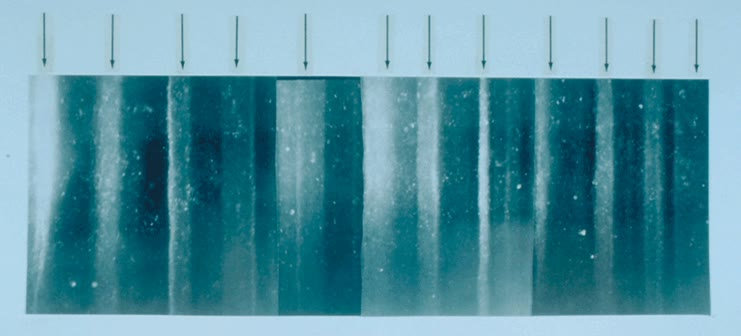
\includegraphics[width=0.72\linewidth]{images/book4/b2-24-gisp2-layers.jpg}
\par\smallskip{\small Une section de la carotte de glace GISP2 du centre du Groenland, prélevée à \qty{1855}{m}
de profondeur, éclairée par-dessous, avec des couches alternées d'été et d'hiver (les flèches sont celles de la diapositive
originale). Pendant l'été nordique sec, la poussière venue du Nord canadien et des côtes du Groenland est
transportée par le vent jusque sur l'inlandsis.
(Anthony Gow, U.S.\ Army Corps of Engineers CRREL, NOAA Paleoclimatology slide set, domaine public,
via Wikimedia Commons.)}
\end{omfigure}
% ledger: photo:b2-24-gisp2, noaa:gisp2-layers

\begin{inthelab}[Découper une carotte de glace]
\begin{minipage}[t]{0.54\linewidth}\vspace{0pt}
Dans un centre national de carottage glaciaire, les carottes sont conservées en tubes, un mètre par tube, dans un
congélateur d'archives à \qty{-36}{\celsius} ; les scientifiques travaillent dans une salle d'examen à
\qty{-24}{\celsius}. À l'arrivée d'une nouvelle carotte, une chaîne de traitement se met en place : scientifiques et
techniciens mesurent, cataloguent et découpent chaque tronçon, à raison de 30 à \qty{35}{m} par jour en moyenne, si bien
qu'une carotte de \qty{1000}{m} demande six à huit semaines. Un chercheur rabote la carotte pour la rendre lisse et mesure
sa conductivité électrique, clé pour définir et dater les couches ; un autre scie les morceaux dont l'air emprisonné sera
analysé pour le dioxyde de carbone et le méthane ; les échantillons sont
ensuite expédiés aux laboratoires qui les mesurent. À EPICA Dome C, chaque échantillon du profil de $\delta$D représentait
\qty{55}{cm} de glace.
\end{minipage}\hfill
\begin{minipage}[t]{0.42\linewidth}\vspace{0pt}
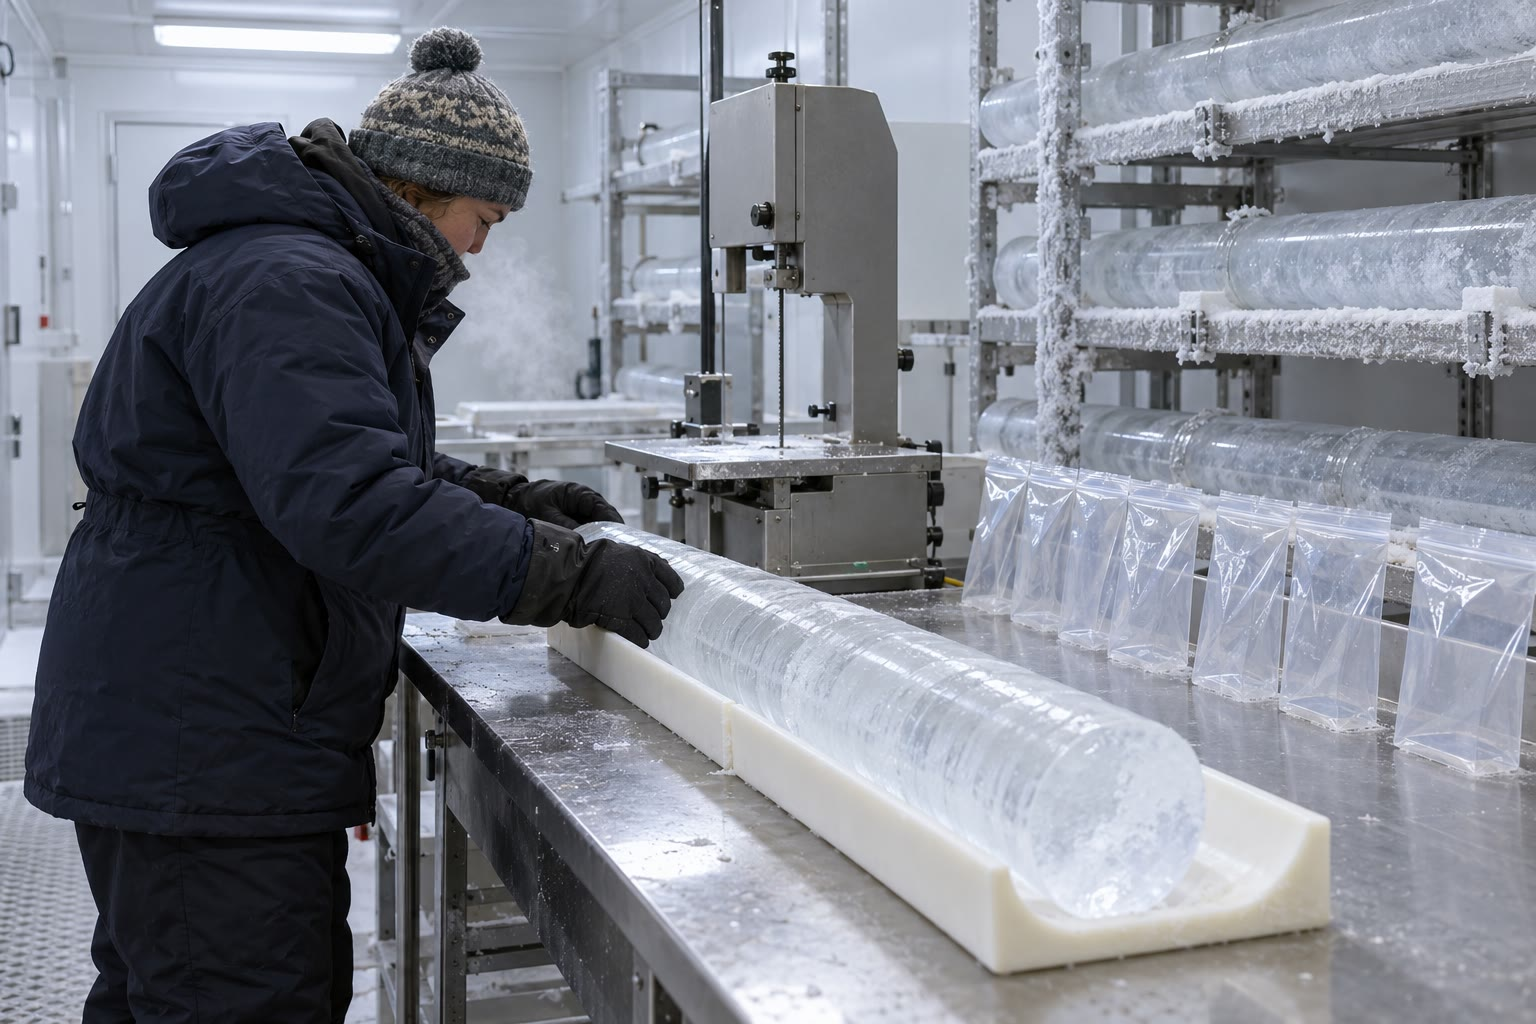
\includegraphics[width=\linewidth]{images/book4/ai/b2-24-cold-lab.jpg}

{\scriptsize Un tronçon de carotte de glace sur la paillasse d'un laboratoire froid, à côté d'une scie à ruban et de sachets
d'échantillons (Illustration générée par IA.)}
\end{minipage}
\end{inthelab}
% ledger: nsficf:cpl, jouzel07:edc-corr

\section{Autres indicateurs, autres archives}\label{sec:b2:climate-proxies:others}

\subsection*{Le magnésium des coquilles}

La calcite des foraminifères fixe un peu de magnésium à la place du calcium, et d'autant plus que
l'eau est plus chaude. Le rapport ne dépend pas de la composition isotopique de l'eau : il donne donc la température
dont l'équation du $\delta^{18}$O a besoin.

\begin{definition}[Rapport Mg/Ca (indicateur)]\label{def:b2:climate-proxies:mgca}
Le \emph{rapport Mg/Ca}\index{rapport Mg/Ca} est le rapport du magnésium au calcium dans
la calcite des coquilles de foraminifères, en \unit{mmol/mol}, utilisée comme mesure de la température de
l'eau dans laquelle la coquille a poussé, au moyen d'une calibration exponentielle
\[
  \text{Mg/Ca} = B\,\mathrm{e}^{A T},
\]
avec $A$ voisin de \qty{0.09}{\per\celsius} pour les espèces planctoniques et $B$ propre à chaque espèce.
\end{definition}
% ledger: groeneveld19:anand, morley24:mgca, miller20:paleotemp

Avec $A = 0.09$, le rapport croît de $\mathrm{e}^{0.09} - 1 = \qty{9.4}{\percent}$ par degré,
quelle que soit la température. Pour une espèce planctonique des eaux froides, la calibration prévue par la seule
température est $\text{Mg/Ca} = 0.4\,\mathrm{e}^{0.09T}$ ; un ajustement sur 235 coquilles issues de filets à plancton
et du sommet de carottes de l'Atlantique Nord donne $0.372\,\mathrm{e}^{0.0936T}$, avec $r^2 = 0.90$.
Aux basses températures, les rapports mesurés s'écartent de la courbe, et cet écart est attribué à la
concentration en ion carbonate de l'eau de mer : un indicateur ne dépend presque jamais d'une seule variable.
Les espèces benthiques sont moins sensibles, d'environ \qty{0.1}{mmol/mol} par degré pour les espèces à faible
teneur en magnésium qui vivent dans le sédiment.
% ledger: morley24:mgca, wharton26:deep

\begin{omfigure}
\centering
% figdata/bachelor-2/proxies.py part calib
\begin{tikzpicture}
\begin{groupplot}[group style={group size=2 by 1, horizontal sep=1.7cm},
  tick label style={font=\scriptsize}, label style={font=\small}, height=5.2cm,
  width=0.48\linewidth]
\nextgroupplot[xmin=-2, xmax=14, ymin=0, ymax=3.8, xlabel={$T$ (\unit{\celsius})},
  ylabel={$\delta^{18}\mathrm{O}_{\mathrm{b}} - \delta^{18}\mathrm{O}_{\mathrm{sw}}$ (pour mille)},
  xtick={0,4,...,12}, title={a\enspace $\delta^{18}$O benthique}, title style={font=\scriptsize}]
\addplot[black, thick] table[x=T, y=dd_benthic] {figdata/out/bachelor-2-proxies-calib.dat};
\nextgroupplot[xmin=0, xmax=30, ymin=0, ymax=6.5, xlabel={$T$ (\unit{\celsius})},
  ylabel={Mg/Ca (\unit{mmol/mol})}, xtick={0,5,...,30}, title={b\enspace Mg/Ca planctonique},
  title style={font=\scriptsize},
  legend style={font=\scriptsize, at={(0.03,0.97)}, anchor=north west, draw=none},
  legend cell align=left]
\addplot[ocRed, thick] table[x=T, y=mgca_pred] {figdata/out/bachelor-2-proxies-calib.dat};
\addlegendentry{$0.4\,\mathrm{e}^{0.09T}$}
\addplot[ocBlue, thick, densely dashed] table[x=T, y=mgca_fit]
  {figdata/out/bachelor-2-proxies-calib.dat};
\addlegendentry{$0.372\,\mathrm{e}^{0.0936T}$}
\end{groupplot}
\end{tikzpicture}
\par\smallskip{\small Deux calibrations. (a) La calibration benthique de la
\cref{prop:b2:climate-proxies:benthic} : la calcite est plus lourde que l'eau (sur leurs échelles propres)
de \num{0.21} pour mille de plus à chaque degré de refroidissement. (b) Le Mg/Ca d'une espèce planctonique,
prévu par la seule température et ajusté sur 235 coquilles.}
\end{omfigure}
% ledger: miller20:paleotemp, morley24:mgca

Mesurés sur les mêmes coquilles, le Mg/Ca et le $\delta^{18}$O donnent deux équations à deux inconnues : le Mg/Ca
donne $T$, et la \cref{prop:b2:climate-proxies:benthic} donne ensuite
$\delta^{18}\mathrm{O}_{\mathrm{sw}}$, le signal de l'\omterm{def:b2:climate-proxies:ice-volume}{effet de volume des glaces}. Appliquée aux coquilles benthiques
de l'Atlantique Nord-Ouest profond, la méthode trouve que l'eau du dernier maximum glaciaire n'était que d'environ
\qty{2}{\celsius} plus froide qu'aujourd'hui ($-1.78 \pm \qty{0.56}{\celsius}$), alors que les estimations issues des
eaux interstitielles placent les deux masses d'eau profondes près du point de congélation dans l'océan glaciaire, $-1.1$ et
\qty{-1.9}{\celsius}, là où elles se trouvent aujourd'hui entre 2 et \qty{4}{\celsius} et entre 0 et \qty{1}{\celsius}.
% ledger: miller20:paleotemp, wharton26:deep

\subsection*{Cernes des arbres}

\begin{definition}[Dendroclimatologie~; interdatation]\label{def:b2:climate-proxies:dendro}
La \emph{dendroclimatologie}\index{dendroclimatologie} est la reconstruction du climat passé à partir des
cernes de croissance annuels des arbres : leur largeur, la densité du bois et leur composition
isotopique. L'\emph{interdatation}\index{interdatation} consiste à faire correspondre le motif des cernes larges et étroits
d'un arbre à l'autre, ce qui attribue à chaque cerne son année calendaire absolue et révèle les cernes
absents localement dans un seul arbre.
\end{definition}
% ledger: bebchuk26:crossdating, bebchuk26:absent-rings, ncei:tree-ring, ncei:proxy

Un cerne est plus large lorsque les conditions favorisent la croissance. L'\omterm{def:b2:climate-proxies:dendro}{interdatation} est fiable dans les sites climatiquement extrêmes, où un seul facteur
climatique limite la croissance de tous les arbres, de sorte qu'ils partagent le même motif ; elle peut échouer là où aucun
facteur ne domine et où de nombreux cernes sont localement absents.
En superposant les motifs des arbres vivants, de vieux bois de charpente et de bois enfouis, on prolonge une chronologie
année par année en remontant le temps ; une étude récente a daté une chronologie de 100 ifs subfossiles de l'est de l'Angleterre
sur les 456 ans allant de 2668 à 2213 av. J.-C., en utilisant le $\delta^{18}$O de plus de \num{1500} de leurs cernes
comparé à une chronologie de chênes datée de façon absolue. L'International Tree-Ring Data Bank conserve les largeurs
et densités des cernes, les isotopes et les chronologies de plus de \num{5000} sites répartis sur six continents.
% ledger: ncei:proxy, bebchuk26:crossdating, bebchuk26:absent-rings, ncei:tree-ring

\subsection*{Grottes et lacs}

\begin{definition}[Spéléothème~; varve]\label{def:b2:climate-proxies:archives}
Un \emph{spéléothème}\index{spéléothème} est un dépôt minéral formé à partir d'eau souterraine dans une
grotte : stalagmites, stalactites et autres formes. Une \emph{varve}\index{varve} est
le dépôt d'une année dans un sédiment de lac ou de fond marin, généralement une paire de lamines de composition
contrastée, l'une déposée en été et l'autre pendant le reste de l'année.
\end{definition}
% ledger: ncei:speleothem, mccarthy23:varves

Les \omterm{def:b2:climate-proxies:archives}{spéléothèmes} croissent couche par couche à partir de l'eau souterraine qui atteint une grotte ; l'épaisseur de leurs couches
et leurs enregistrements isotopiques donnent les conditions climatiques passées. Certains sont annuellement rubanés,
et d'autres renferment des composés datables par radiométrie. L'échelle de temps des carottes du Groenland concorde avec celle
des \omterm{def:b2:climate-proxies:archives}{spéléothèmes} de la grotte de Hulu à 800 ans près sur les \num{60000} dernières années : deux
archives, datées par des méthodes différentes, se contrôlent mutuellement.
% ledger: ncei:speleothem, svensson08:gicc05

\begin{omfigure}
\centering
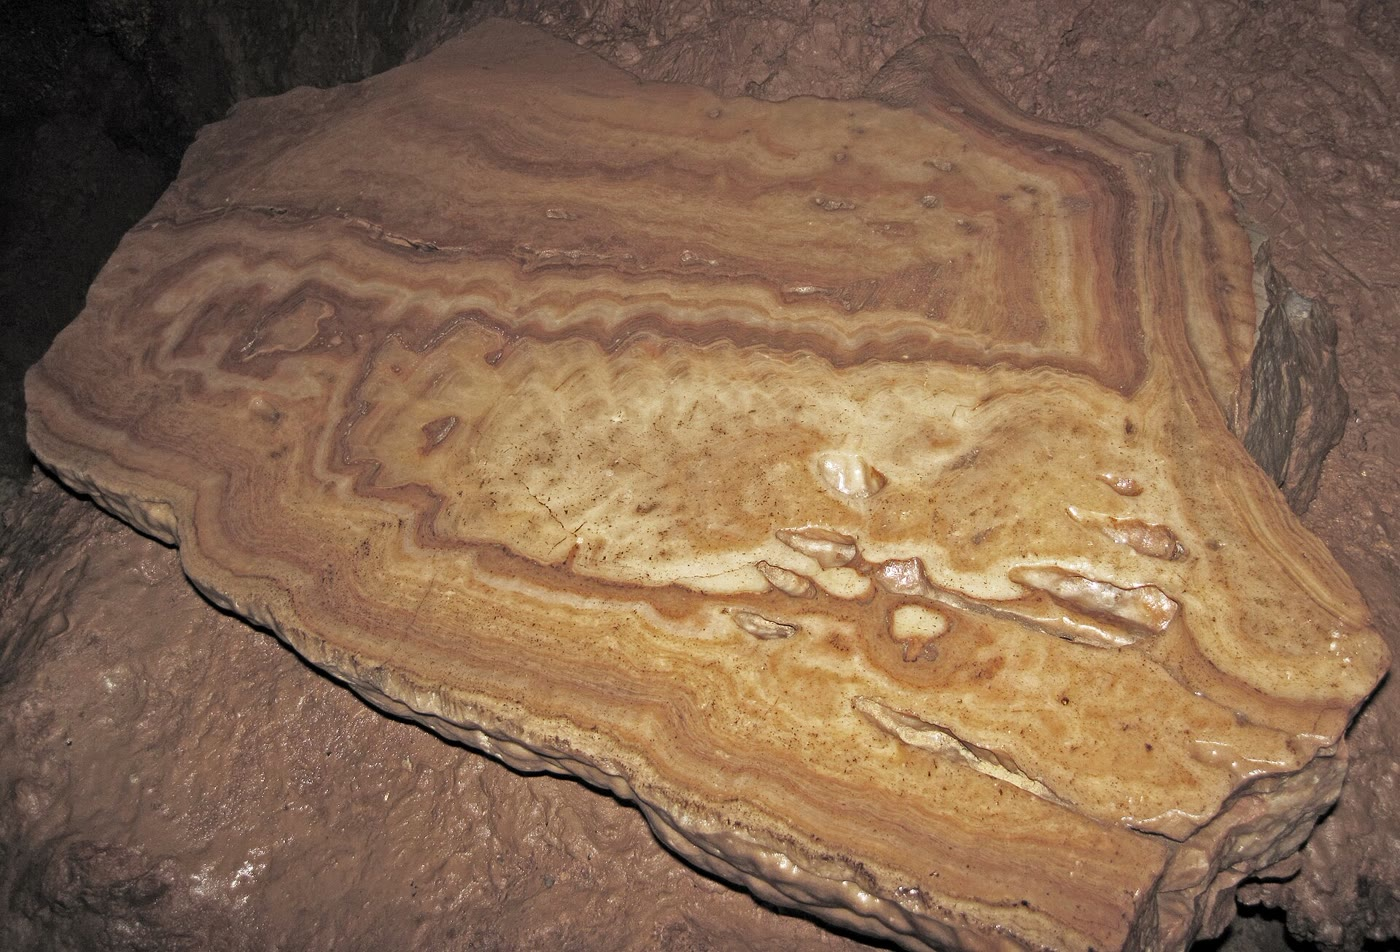
\includegraphics[width=0.62\linewidth]{images/book4/b2-24-speleothem.jpg}
\par\smallskip{\small Coupe polie d'un \omterm{def:b2:climate-proxies:archives}{spéléothème} de calcite provenant de Diamond Caverns,
Kentucky, colorée par des impuretés d'oxydes de fer : chaque bande fut jadis la surface du dépôt.
(James St.~John, CC BY 2.0, via Wikimedia Commons.)}
\end{omfigure}
% ledger: photo:b2-24-speleothem

Dans le bassin profond du lac Crawford, en Ontario, l'eau de fond, plus salée et plus alcaline que l'eau qui la surmonte,
ne contient aucun animal assez gros pour remuer la vase ; bien qu'elle soit bien oxygénée, elle reçoit chaque année un couplet :
une couche de matière organique, coiffée par la calcite qui précipite chaque été à partir de l'eau de surface alcaline.
Les sédiments lacustres conservent aussi le pollen de la végétation environnante, lu par analyse pollinique ;
varvés ou non, ils enregistrent
le territoire.
% ledger: mccarthy23:varves, mccarthy23:no-bioturbation, ncei:pollen

\section{Modèles d'âge}\label{sec:b2:climate-proxies:age}

Un indicateur sans date n'est qu'une curiosité. Toute archive exige une relation entre la profondeur, ou le cerne, ou la
bande, et l'âge.

\begin{definition}[Modèle d'âge~; comptage des couches annuelles]\label{def:b2:climate-proxies:age-model}
Un \emph{modèle d'âge}\index{modèle d'âge} est la fonction qui affecte un âge, avec son incertitude, à
chaque profondeur d'une archive. Le \emph{comptage des couches annuelles}\index{comptage des couches annuelles} construit un modèle d'âge
en comptant, de haut en bas, les couches qui enregistrent chacune une année (couches de glace, \omterm{def:b2:climate-proxies:archives}{varves},
bandes), chaque couche dont le caractère annuel est douteux étant comptée comme une demi-année, plus ou moins
une demi-année.
\end{definition}
% ledger: svensson08:gicc05, mccarthy23:varves

\begin{method}[Construire un modèle d'âge]\label{met:b2:climate-proxies:age-model}
\begin{enumerate}
  \item Lorsque l'archive possède des couches annuelles, les compter depuis un sommet connu, en notant à part
        les incertaines.
  \item Lorsqu'elle n'en a pas, ou qu'elles ne se laissent pas résoudre, fixer des \emph{points de calage} : des profondeurs
        datées indépendamment, par radiocarbone ou une autre méthode radiométrique, par une cendre volcanique datée, ou en
        faisant correspondre un enregistrement bien daté.
  \item Entre les points de calage, interpoler, linéairement en profondeur si rien de mieux n'est connu, ou à l'aide
        d'un modèle de la manière dont l'archive s'est accumulée et amincie.
  \item Reporter l'incertitude de chaque étape sur toutes les profondeurs.
\end{enumerate}
\end{method}
% ledger: svensson08:gicc05, noaa:gisp2-layers, ncei:speleothem

La Greenland Ice Core Chronology 2005, GICC05, compte les couches annuelles dans trois carottes du Groenland, et
dans la partie glaciaire de la seule carotte NorthGRIP, sur les \num{60000} dernières années ; ses âges sont
donnés en années avant 2000 de notre ère, notées b2k. Les couches incertaines, comptées comme $\frac12 \pm \frac12$,
s'additionnent pour donner l'\emph{erreur maximale de comptage}, que les auteurs
considèrent comme deux écarts types. Au début de l'Holocène, 11\,703 ans b2k, elle vaut 50 ans ;
au début de l'interstade groenlandais 17, \num{59440} ans b2k, elle vaut \num{1287} ans.
% ledger: svensson08:gicc05, svensson08:table1

\begin{proposition}[Croissance d'une erreur de comptage]\label{prop:b2:climate-proxies:counting}
Soit un comptage contenant $n$ couches incertaines, chacune comptée comme $\frac12$ avec une erreur d'écart type
$\frac12$. Si les erreurs des couches sont indépendantes, l'écart type du total est
$\frac12\sqrt{n}$ ; si elles sont toutes de même signe, l'erreur du total est
$\frac12 n$.
\end{proposition}

\begin{proof}
La variance d'une somme d'erreurs indépendantes est la somme de leurs variances : $n \times
(\frac12)^2$, dont la racine carrée vaut $\frac12\sqrt{n}$. Si chaque couche se trompe de la même façon, les
erreurs s'additionnent comme des nombres : $n \times \frac12$.
\end{proof}

À GI-17, les \num{1287} ans d'erreur maximale de comptage représentent \num{2574} couches incertaines. Si
leurs erreurs étaient indépendantes, le total ne serait incertain que de $\frac12\sqrt{2574} = 25$ ans.
La somme linéaire est le choix prudent : les couches douteuses d'un même intervalle de glace sont jugées par
les mêmes compteurs selon les mêmes critères, et rien ne permet d'attendre que leurs erreurs se compensent.
La partie ancienne de l'enregistrement a été comptée indépendamment par deux des auteurs ; leurs comptages
diffèrent de moins que l'erreur absolue, mais localement de plus que l'erreur finale de comptage. L'erreur
maximale de comptage vaut en moyenne environ \qty{1}{\percent} de la durée d'une section dans l'Holocène et
\qty{5}{\percent} dans la partie glaciaire.
% ledger: svensson08:gicc05, svensson08:table1, svensson08:two-counters

\begin{omfigure}
\centering
% figdata/bachelor-2/proxies.py part gicc05
\begin{tikzpicture}
\begin{groupplot}[group style={group size=2 by 1, horizontal sep=1.7cm},
  tick label style={font=\scriptsize}, label style={font=\small}, height=5.4cm,
  width=0.48\linewidth, xmin=0, xmax=62, xlabel={âge GICC05 (\unit{ka} b2k)}]
\nextgroupplot[ymin=1450, ymax=2450, y dir=reverse, ylabel={profondeur NorthGRIP (\unit{m})},
  title={a\enspace profondeur et âge}, title style={font=\scriptsize}]
\addplot[black, mark=*, mark size=1.1pt] table[x=age_ka, y=depth_m]
  {figdata/out/bachelor-2-proxies-gicc05.dat};
\nextgroupplot[ymode=log, ymin=2, ymax=30000, ylabel={incertitude (années)},
  title={b\enspace incertitude de comptage}, title style={font=\scriptsize},
  legend style={font=\scriptsize, at={(0.03,0.97)}, anchor=north west, draw=none},
  legend cell align=left]
\addplot[ocRed, mark=*, mark size=1.1pt] table[x=age_ka, y=err_yr]
  {figdata/out/bachelor-2-proxies-gicc05.dat};
\addlegendentry{erreur maximale de comptage}
\addplot[ocBlue, mark=o, mark size=1.1pt] table[x=age_ka, y=err_random_yr]
  {figdata/out/bachelor-2-proxies-gicc05.dat};
\addlegendentry{si indépendantes}
\end{groupplot}
\end{tikzpicture}
\par\smallskip{\small La chronologie GICC05 aux 18 événements climatiques, du début de l'Holocène à \qty{59.44}{ka} :
(a) profondeur dans la carotte NorthGRIP en fonction de l'âge ; la courbe s'aplatit parce que les couches annuelles
s'amincissent avec la profondeur, chaque millier d'années occupant de moins en moins de mètres de glace ;
(b) l'erreur maximale de comptage, et l'erreur que donneraient les mêmes couches incertaines si leurs erreurs étaient indépendantes
(\cref{prop:b2:climate-proxies:counting}) ; échelle logarithmique. Données~: Svensson et al.\ (2008), tableau 1.}
\end{omfigure}
% ledger: svensson08:table1, svensson08:gicc05

Les couches annuelles s'amincissent avec la profondeur, parce que la glace coule et s'étale en s'enfonçant : entre le début de
l'Holocène et GI-1, la couche moyenne mesure \qty{3.75}{cm} d'épaisseur dans NorthGRIP ; entre GI-16 et
GI-17, \qty{1.54}{cm} ; vers \qty{100}{ka}, les modèles d'écoulement la placent près de \qty{1}{cm}. Plus les couches sont minces, plus il est difficile de les distinguer
les unes des autres.
% ledger: svensson08:table1, svensson08:gicc05

\section{Calibration}\label{sec:b2:climate-proxies:calibration}

Tout nombre lu sur un indicateur passe par une calibration.

\begin{definition}[Calibration d'un indicateur]\label{def:b2:climate-proxies:calibration}
Une \emph{calibration d'un indicateur}\index{calibration d'un indicateur} est la relation empirique ou théorique qui
convertit la valeur d'un indicateur en la variable climatique qu'il représente, établie sur des échantillons pour
lesquels les deux grandeurs sont connues, avec son incertitude et la plage de conditions dans laquelle elle est
valable.
\end{definition}
% ledger: morley24:mgca, miller20:paleotemp

Les échantillons pour lesquels les deux grandeurs sont connues sont actuels : coquilles recueillies dans des filets à plancton, sommets de carottes de sédiment comparés à l'eau qui les surmonte, neige récente comparée à la
température de son site, cernes externes des arbres comparés aux relevés d'une station météorologique.
La relation est ensuite ajustée par moindres carrés ; pour une loi exponentielle comme la calibration du Mg/Ca,
l'ajustement se fait sur le logarithme, ce qui transforme $\text{Mg/Ca} = B\,\mathrm{e}^{AT}$ en
la droite $\ln(\text{Mg/Ca}) = \ln B + AT$. Une calibration se valide sur des échantillons qui n'ont pas servi à l'ajuster :
une part des données actuelles est mise de côté, puis prédite.
% ledger: morley24:mgca, werner18:slopes, ncei:tree-ring

Trois limites subsistent. Une calibration mesurée dans l'espace, d'un lieu à l'autre aujourd'hui, peut ne pas tenir
dans le temps, comme l'a montré la glace du Groenland.
Une calibration mesurée sur l'étendue actuelle des conditions
doit être extrapolée avec prudence : le Mg/Ca des coquilles s'écarte de sa loi aux basses températures, là où une autre variable,
l'ion carbonate, prend le relais. Et une relation linéaire sur un petit intervalle peut ne pas l'être sur un grand, comme
l'\omterm{def:b2:climate-proxies:ice-volume}{effet de volume des glaces} ne l'est pas. La méthode de ce chapitre répond à ces limites de la même façon :
mesurer deux indicateurs indépendants sur un même échantillon, et laisser chacun contrôler l'autre.
% ledger: werner18:slopes, morley24:mgca, rohling21:linear

\section*{Exercices}\label{sec:b2:climate-proxies:exercises}

Données des exercices, sauf indication contraire : profondeur moyenne de l'océan $H = \qty{3682.2}{m}$, surface océanique
\qty{361.84e6}{km^2} ; la calibration benthique de la \cref{prop:b2:climate-proxies:benthic} ; la calibration
planctonique $\text{Mg/Ca} = 0.4\,\mathrm{e}^{0.09T}$ (\unit{mmol/mol}, \unit{\celsius}) ;
valeurs $\delta$ des eaux et de la glace en pour mille \omterm{def:b2:isotope-geochemistry:standards}{VSMOW}, et de la calcite en pour mille \omterm{def:b2:isotope-geochemistry:standards}{VPDB}.
% ledger: charette:ocean-volume, miller20:paleotemp, morley24:mgca

\begin{exercise}[$\star$]\label{exo:b2:climate-proxies:1}
Aujourd'hui, la glace continentale renferme environ \qty{27.5e6}{km^3} et l'océan \qty{1350e6}{km^3} d'eau
(on prendra les volumes comme des quantités d'eau). (a) Si la glace a un $\delta^{18}$O moyen de $-30$ pour
mille et l'océan 0, quel est le $\delta^{18}$O de l'hydrosphère entière, en négligeant l'eau douce~?
(b) Si toute la glace fondait, quel serait le $\delta^{18}$O de l'océan~? (c) Quelle fraction
de l'eau est de la glace~?
\end{exercise}
% ledger: white13c9:ice-mass

\begin{exercise}[$\star$]\label{exo:b2:climate-proxies:2}
Une coquille benthique a $\delta^{18}\mathrm{O}_{\mathrm{b}} = 2.50$ pour mille. (a) Calculer sa
température si l'eau de mer avait $\delta^{18}\mathrm{O}_{\mathrm{sw}} = 0$. (b) La calculer si l'eau de mer avait
$+1.0$ pour mille. (c) Une autre coquille, issue de la même eau à $0$ pour mille, a
$2.71$ pour mille : de combien son eau était-elle plus froide~?
\end{exercise}
% ledger: miller20:paleotemp

\begin{exercise}[$\star$]\label{exo:b2:climate-proxies:3}
(a) Calculer le \omterm{def:b2:climate-proxies:mgca}{rapport Mg/Ca} de la calibration planctonique à \qty{10}{\celsius} et à
\qty{20}{\celsius}. (b) De quel facteur le rapport croît-il sur ces dix degrés, et de quel
pourcentage par degré~? (c) Calculer la température de coquilles de Mg/Ca = 2.0 et
\qty{1.0}{mmol/mol}.
\end{exercise}
% ledger: morley24:mgca

\begin{exercise}[$\star$]\label{exo:b2:climate-proxies:4}
Une chronologie d'ifs subfossiles s'étend de 2668 à 2213 av. J.-C. (a) Sur combien d'années s'étend-elle,
en comptant les deux années extrêmes~? (b) Pourquoi une chronologie construite à partir de nombreux arbres mérite-t-elle plus de
confiance que le comptage des cernes d'un seul arbre~? (c) Pourquoi attendre de l'\omterm{def:b2:climate-proxies:dendro}{interdatation} qu'elle soit plus facile pour
des arbres proches de la limite arborée, en climat froid, que pour des arbres d'une forêt de plaine douce et humide~?
\end{exercise}
% ledger: bebchuk26:crossdating

\begin{exercise}[$\star\star$]\label{exo:b2:climate-proxies:5}
(a) Avec la \cref{prop:b2:climate-proxies:mass-balance}, calculer l'\omterm{def:b2:climate-proxies:ice-volume}{effet de volume des glaces} pour une baisse
du niveau de la mer de \qty{125}{m} et de \qty{134}{m}, avec une glace à $-40$ pour mille. (b) Le calculer pour
\qty{130}{m} avec une glace à $-30$, $-35$ et $-50$ pour mille. (c) Quelle composition moyenne de la glace
ferait que l'effet d'une baisse de \qty{130}{m} égale le \num{1.0} pour mille mesuré dans les eaux
interstitielles~? Comparer avec les compositions des inlandsis actuels.
\end{exercise}
% ledger: ipcc:lgm-sea, white:d18o, miller20:ice-cal, wharton26:deep

\begin{exercise}[$\star\star$]\label{exo:b2:climate-proxies:6}
Comparer les deux calibrations du Mg/Ca de la même espèce planctonique : celle prévue par la seule
température, $0.4\,\mathrm{e}^{0.09T}$, et l'ajustement $0.372\,\mathrm{e}^{0.0936T}$. (a) À quelle
température s'accordent-elles~? (b) À \qty{2}{\celsius}, de quel pourcentage le rapport ajusté est-il inférieur
au rapport prévu~? (c) Une coquille formée à \qty{2}{\celsius} suit la loi ajustée ; quelle température la loi prévue
lui donnerait-elle~?
\end{exercise}
% ledger: morley24:mgca

\begin{exercise}[$\star\star$]\label{exo:b2:climate-proxies:7}
Dans la carotte NorthGRIP, le début de l'Holocène se trouve à \qty{1492.45}{m} et \num{11703} ans
b2k, le début de GI-1 à \qty{1604.64}{m} et \num{14692} ans ; le début de GI-16 à
\qty{2402.55}{m} et \num{58280} ans, celui de GI-17 à \qty{2420.44}{m} et \num{59440} ans.
(a) Calculer l'épaisseur moyenne des couches annuelles dans chaque intervalle. (b) Pourquoi sont-elles plus minces
plus profondément~? (c) Pourquoi le \omterm{def:b2:climate-proxies:age-model}{comptage des couches annuelles} devient-il impossible à partir d'une certaine profondeur~?
\end{exercise}
% ledger: svensson08:table1, svensson08:gicc05

\begin{exercise}[$\star\star$]\label{exo:b2:climate-proxies:8}
Utiliser les deux premiers points de calage de l'\cref{exo:b2:climate-proxies:7}, avec des erreurs maximales de comptage de 50
et 93 ans. (a) Par interpolation linéaire en profondeur, donner l'âge de la glace à \qty{1550}{m}.
(b) L'exprimer en années avant 1950. (c) Interpoler l'incertitude de la même façon.
\end{exercise}
% ledger: svensson08:table1

\begin{exercise}[$\star\star$]\label{exo:b2:climate-proxies:9}
L'erreur maximale de comptage de GICC05 est de 93 ans à GI-1 et de \num{1287} ans à GI-17. (a) Combien de
couches incertaines représente chacune~? (b) Quelle serait l'incertitude si les erreurs de ces couches étaient
indépendantes, chacune d'écart type une demi-année~? (c) De quel facteur la somme linéaire dépasse-t-elle l'estimation
indépendante dans chaque cas, et pourquoi ce facteur croît-il avec la profondeur~?
\end{exercise}
% ledger: svensson08:gicc05, svensson08:table1

\begin{exercise}[$\star\star\star$]\label{exo:b2:climate-proxies:10}
À EPICA Dome C, le $\delta$D moyen de la glace vaut $-396.6$ pour mille sur les deux derniers milliers d'années
et $-441.7$ pour mille sur 19 à \qty{23}{ka}. (a) La pente spatiale antarctique de $\delta^{18}$O vaut
\num{0.8} pour mille par degré. Avec la \omterm{prop:b2:isotope-geochemistry:mwl}{droite des eaux météoriques}, la convertir en pente de $\delta$D et
estimer le refroidissement glaciaire. (b) L'océan glaciaire était de \num{1.0} pour mille plus lourd en
$\delta^{18}$O, de sorte que la neige qui s'y est formée était plus lourde elle aussi. En supposant que le $\delta$D de l'océan
a varié huit fois autant, corriger le $\delta$D glaciaire et estimer de nouveau le refroidissement.
(c) L'anomalie publiée vaut $-0.09$ et \qty{-9.39}{\celsius} pour les deux périodes ; quelle pente de
$\delta$D par degré cela implique-t-il, et quelle autre correction la série publiée contient-elle~?
\end{exercise}
% ledger: data:b4-proxies, werner18:slopes, kc98:mwl, wharton26:deep, jouzel07:edc-corr

\begin{exercise}[$\star\star\star$]\label{exo:b2:climate-proxies:11}
Une calibration du Mg/Ca d'une espèce planctonique utilise six échantillons de sommets de carottes (température de l'eau,
Mg/Ca en \unit{mmol/mol}) : (4, 0.59), (8, 0.80), (12, 1.21), (16, 1.65), (20, 2.47), (24, 3.41).
(a) Ajuster $\ln(\text{Mg/Ca}) = \ln B + AT$ par moindres carrés, et donner $A$ et $B$. (b) Calculer les
résidus du logarithme, et comparer l'ajustement à la loi $0.4\,\mathrm{e}^{0.09T}$. (c) Donner la
température d'une coquille glaciaire de Mg/Ca = 1.30. (d) Une coquille a un Mg/Ca = 0.45 : calculer sa
température, et dire pourquoi cette valeur mérite moins confiance que la précédente.
\end{exercise}
% ledger: morley24:mgca

\begin{exercise}[$\star\star\star$]\label{exo:b2:climate-proxies:12}
Un inlandsis croît en deux temps : d'abord \qty{60}{m} de niveau de la mer sont stockés sous forme de glace à $-30$ pour
mille, puis \qty{70}{m} de plus sous forme de glace à $-45$ pour mille. (a) Montrer que le bilan de masse de
la \cref{prop:b2:climate-proxies:mass-balance} devient $(H - h)\,\Delta\delta = -\sum_i h_i\delta_i$
pour plusieurs réserves de glace, et calculer l'\omterm{def:b2:climate-proxies:ice-volume}{effet de volume des glaces} après chaque étape. (b) Quelle est la
composition moyenne de la glace à la fin~? (c) Une règle linéaire, calibrée sur l'état final, convertit
$\Delta\delta$ en niveau de la mer. Quelle baisse du niveau de la mer en déduirait-elle pour la première étape, et pourquoi
se trompe-t-elle~?
\end{exercise}
% ledger: rohling21:linear, white:d18o, miller20:ice-cal

\begin{problem}[{Problème du week-end --- Une coquille, deux signaux}]\label{pb:b2:climate-proxies:1}
De combien le fond de l'océan était-il plus froid au dernier maximum glaciaire~? Le $\delta^{18}$O des coquilles benthiques
mêle la réponse au volume de la glace ; ce problème sépare les deux. Utiliser les données des exercices ; le niveau de la mer
était de 125 à \qty{134}{m} plus bas qu'aujourd'hui, et la glace de l'inlandsis nord-américain aurait eu
un $\delta^{18}$O d'environ $-40$ pour mille.

\medskip\noindent\textbf{Partie I --- La glace sur les continents.}
\begin{enumerate}
  \item Calculer le volume d'eau retiré de l'océan par une baisse du niveau de la mer de \qty{130}{m}.
  \item Calculer l'\omterm{def:b2:climate-proxies:ice-volume}{effet de volume des glaces} de cette baisse, avec une glace à $-40$ pour mille.
  \item Le calculer pour des baisses de \qty{125}{m} et de \qty{134}{m}.
  \item Le calculer pour \qty{130}{m} avec une glace à $-35$ et à $-50$ pour mille. Quelle incertitude
        pèse le plus, celle du niveau de la mer ou celle de la glace~?
  \item Les eaux interstitielles des sédiments glaciaires donnent $1.0 \pm 0.1$ pour mille. Quelle composition moyenne
        de la glace une baisse de \qty{130}{m} exigerait-elle pour le produire~?
  \item Calculer le décalage par mètre de niveau de la mer pour de petites baisses avec une glace à $-40$ pour mille, et
        comparer avec la valeur de \num{0.011} pour mille par mètre déduite des niveaux marins datés.
\end{enumerate}

\medskip\noindent\textbf{Partie II --- Deux thermomètres.}
\begin{enumerate}[resume]
  \item Montrer à partir de la \cref{prop:b2:climate-proxies:benthic} qu'un refroidissement de \qty{1}{\celsius} à composition d'eau constante élève
        $\delta^{18}\mathrm{O}_{\mathrm{b}}$ de \num{0.21} pour mille.
  \item Calculer $\delta^{18}\mathrm{O}_{\mathrm{b}}$ d'une coquille benthique formée aujourd'hui dans une eau à
        \qty{2.0}{\celsius} avec $\delta^{18}\mathrm{O}_{\mathrm{sw}} = 0$.
  \item Le calculer pour une coquille glaciaire formée dans une eau à \qty{-1.0}{\celsius} avec
        $\delta^{18}\mathrm{O}_{\mathrm{sw}} = +1.0$ pour mille. Quelle est la variation entre les deux
        coquilles, et quelle part en revient à la composition de l'eau~?
  \item Une coquille planctonique a un Mg/Ca de \qty{2.0}{mmol/mol}. Calculer sa température.
  \item Les coquilles benthiques à faible teneur en magnésium gagnent environ \qty{0.1}{mmol/mol} par degré. Une coquille glaciaire a
        un Mg/Ca inférieur de \qty{0.18}{mmol/mol} à celui d'une coquille actuelle de la même espèce et du même lieu.
        Quel refroidissement cela indique-t-il~?
  \item Pourquoi le Mg/Ca donne-t-il une température qui ne dépend pas du volume de la glace~?
\end{enumerate}

\medskip\noindent\textbf{Partie III --- Le résidu.}
La compilation LR04 vaut \num{3.23} pour mille aujourd'hui et \num{4.92} pour mille en moyenne sur 19 à
\qty{23}{ka}.
\begin{enumerate}[resume]
  \item Calculer la variation de la compilation entre aujourd'hui et le dernier maximum glaciaire.
  \item Si toute cette variation était due à l'\omterm{def:b2:climate-proxies:ice-volume}{effet de volume des glaces}, avec une glace à $-40$ pour mille, quelle baisse du niveau
        de la mer en résulterait-elle (inverser la \cref{prop:b2:climate-proxies:mass-balance}) ? Est-ce compatible avec
        les indices de niveau de la mer~?
  \item Prendre l'\omterm{def:b2:climate-proxies:ice-volume}{effet de volume des glaces} de la question 2. Quel résidu reste pour la température, et quel refroidissement
        de l'eau profonde en résulte-t-il~?
  \item Prendre plutôt la valeur de l'eau interstitielle, \num{1.0} pour mille. Quel résidu et quel refroidissement~?
  \item Une autre reconstitution utilise \num{0.25} pour mille par degré. Refaire les deux estimations avec celle-ci.
  \item Aujourd'hui, l'eau profonde nord-atlantique est entre 2 et \qty{4}{\celsius} et l'eau de fond antarctique
        est entre 0 et \qty{1}{\celsius} ; les eaux interstitielles les placent à $-1.1$ et \qty{-1.9}{\celsius}
        dans l'océan glaciaire, et le Mg/Ca des coquilles benthiques ne trouve l'Atlantique Nord-Ouest profond que
        d'environ \qty{1.8}{\celsius} plus froid. Quelle plage de refroidissement ces valeurs donnent-elles, et laquelle des
        deux estimations des questions 15 et 16 favorisent-elles~?
\end{enumerate}

\medskip\noindent\textbf{Partie IV --- La vue depuis la glace.}
À EPICA Dome C, le $\delta$D moyen vaut $-396.6$ pour mille sur les deux derniers milliers d'années et
$-441.7$ pour mille sur 19 à \qty{23}{ka} ; l'anomalie de température publiée vaut $-0.09$ et
\qty{-9.39}{\celsius}.
\begin{enumerate}[resume]
  \item Calculer la variation de $\delta$D.
  \item Avec une pente de $\delta^{18}$O de \num{0.8} pour mille par degré et la \omterm{prop:b2:isotope-geochemistry:mwl}{droite des eaux météoriques}, estimer
        le refroidissement à Dome C.
  \item Calculer le refroidissement publié, et la pente de $\delta$D par degré qu'il implique.
  \item La température moyenne de la surface du globe était inférieure de 5 à \qty{7}{\celsius} au dernier maximum glaciaire.
        Classer les refroidissements de Dome C, du globe et de l'océan profond.
  \item Pourquoi l'océan profond n'a-t-il pas pu se refroidir autant que la surface de l'Antarctique~?
  \item En résumé : avec la correction de l'eau interstitielle pour l'\omterm{def:b2:climate-proxies:ice-volume}{effet de volume des glaces}, de combien l'océan profond
        était-il plus froid au dernier maximum glaciaire qu'aujourd'hui~?
\end{enumerate}
\end{problem}
% ledger: charette:ocean-volume, ipcc:lgm-sea, miller20:ice-cal, white:d18o, white13c9:ice-volume, wharton26:deep, miller20:paleotemp, morley24:mgca, data:b4-proxies, rohling21:linear, werner18:slopes, kc98:mwl, ipcc:lgm-cooling
